\newpage

\section{Trigonometrie}
\subsection{Gradmass, Bogenmass}
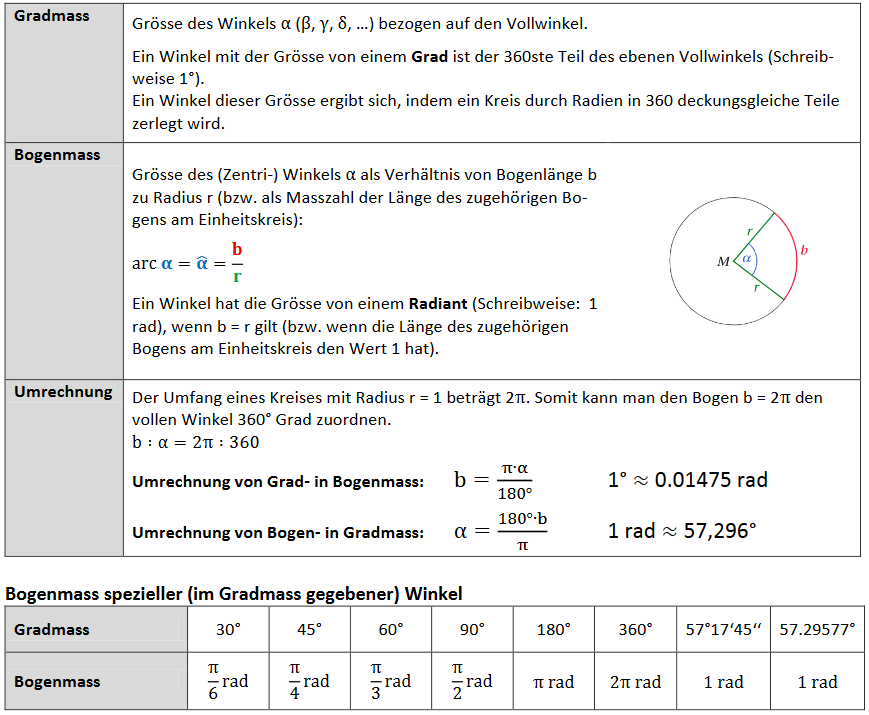
\includegraphics[scale=0.7]{gradmass.PNG}
\subsection{Trigonometrische Funktionen am rechtwinkligen Dreieck}
\subsubsection{Sinus, Kosekans}
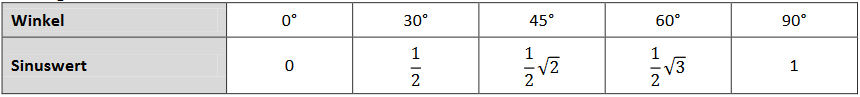
\includegraphics[scale=0.7]{sinkan1.PNG}

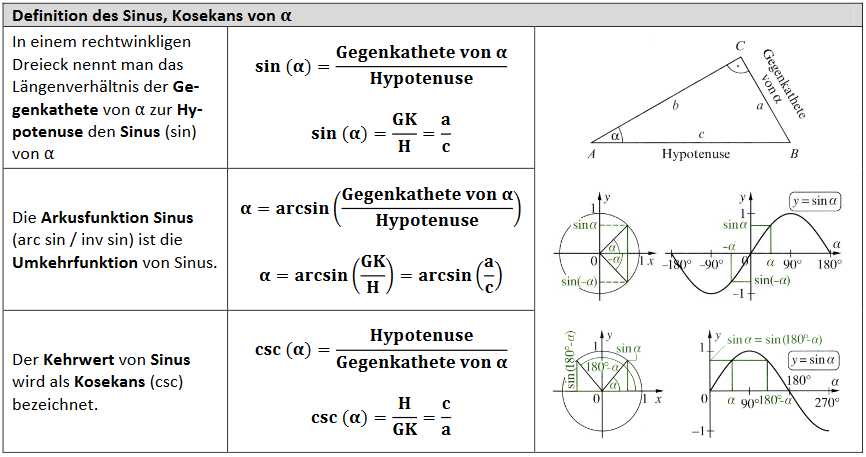
\includegraphics[scale=0.7]{sinkan2.PNG}
\subsubsection{Kosinus, Sekans}
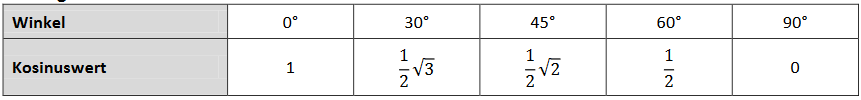
\includegraphics[scale=0.7]{kossek1.PNG}

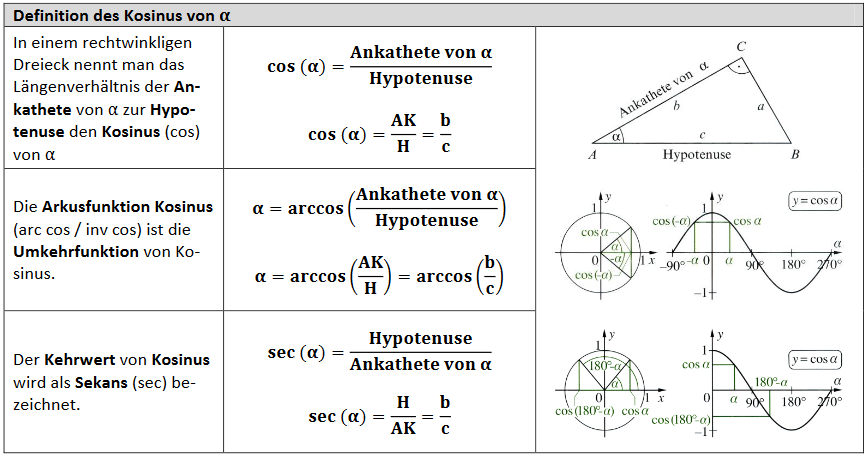
\includegraphics[scale=0.7]{kossek2.PNG}
\subsubsection{Tangens, Kotangens}
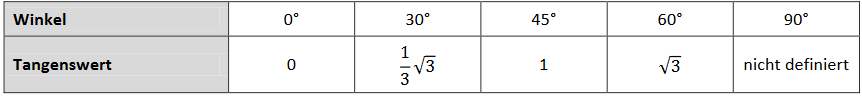
\includegraphics[scale=0.7]{tanko1.PNG}

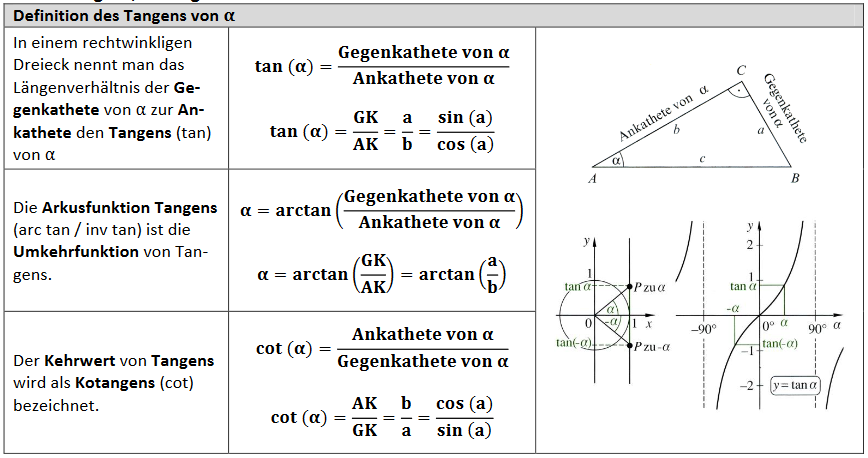
\includegraphics[scale=0.7]{tanko2.PNG}

\subsubsection{Sinus- Kosinus- und Tangensfunktion am rechtwinkligen Dreieck}
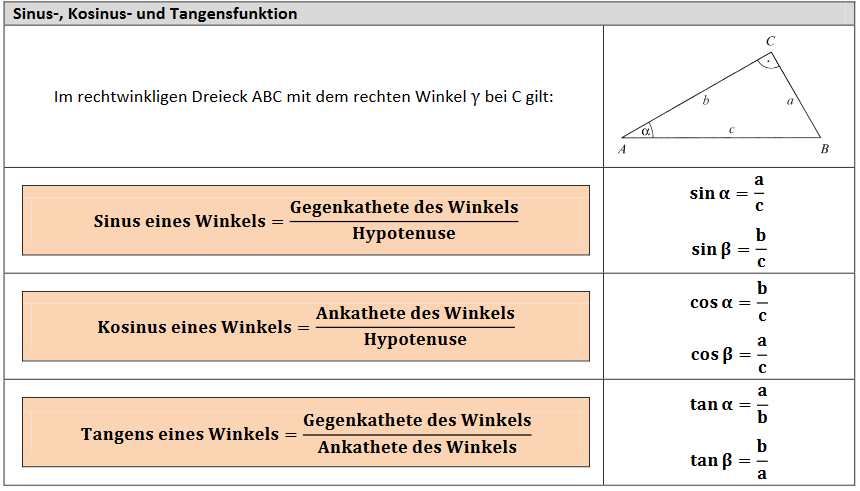
\includegraphics[scale=0.7]{sinkota.PNG}

\newpage{}


\subsection{Trigonometrische Funktionen am schiefwinkligen Dreieck}
\subsubsection{Kosinussatz}
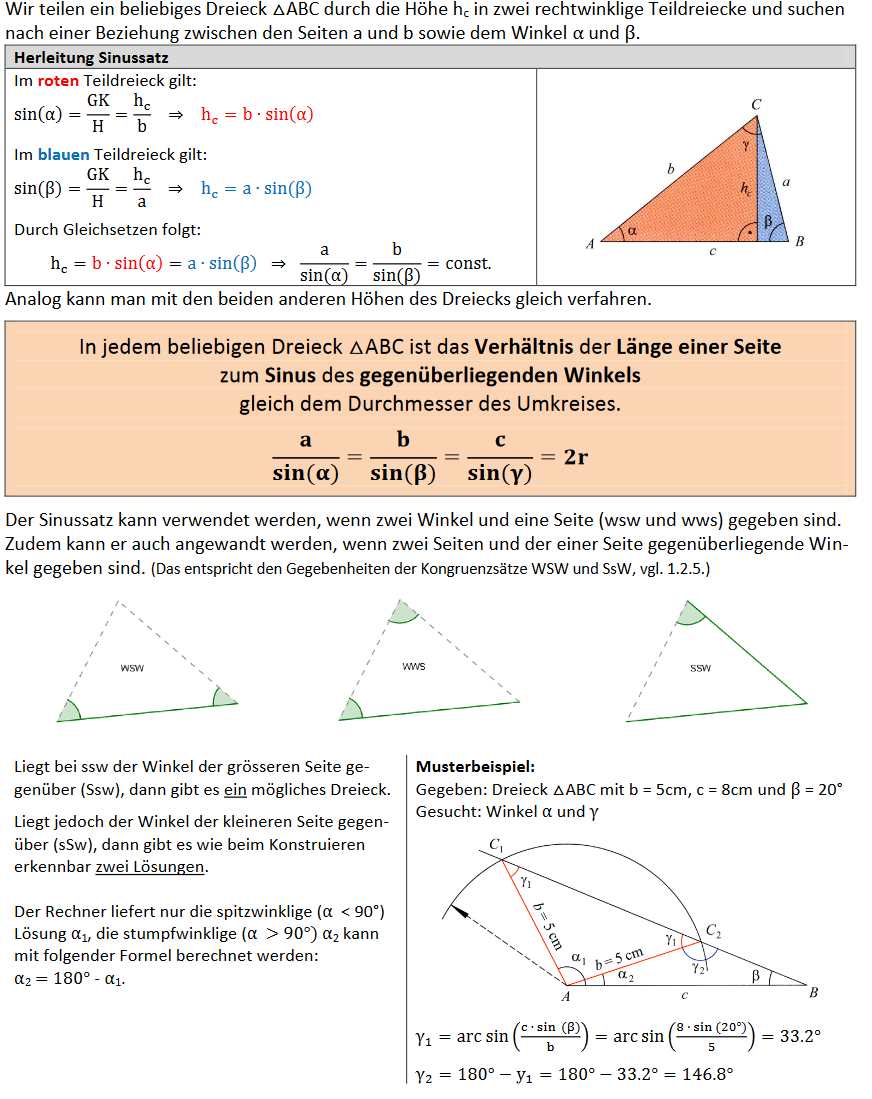
\includegraphics[scale=0.7]{sinussatz.PNG}
\subsubsection{Sinussatz}
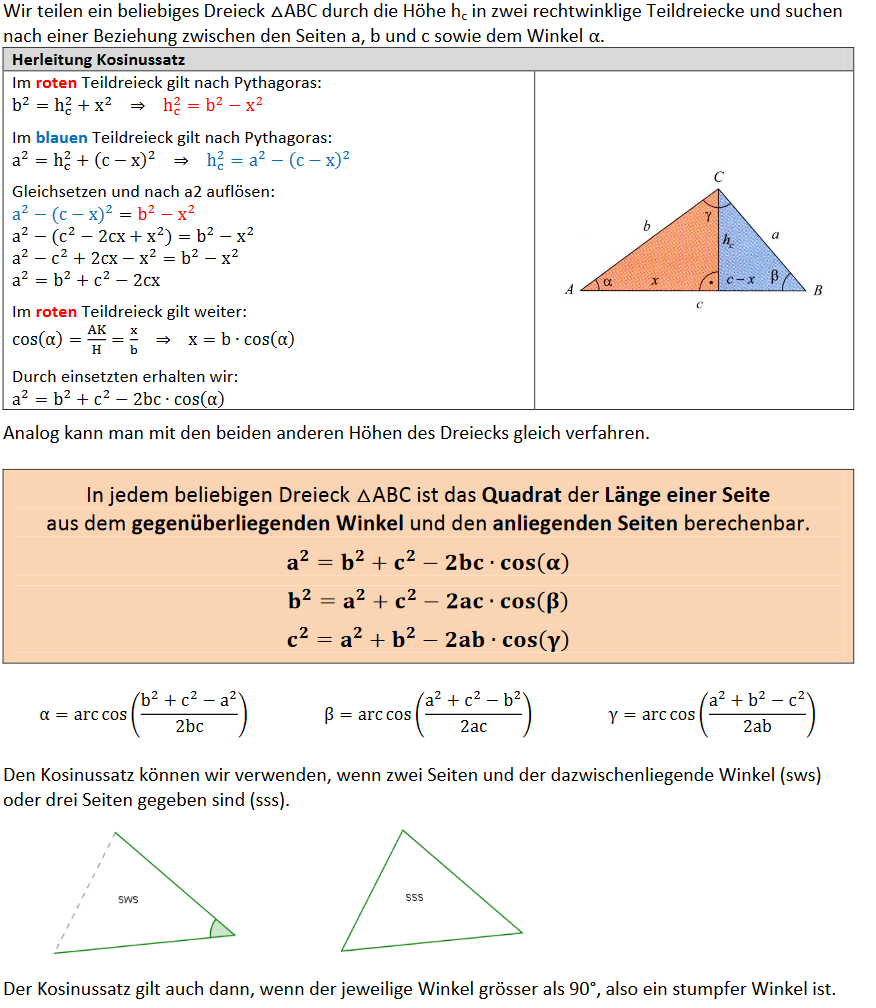
\includegraphics[scale=0.7]{kosinussatz.PNG}

\subsubsection{Flaechensatz}
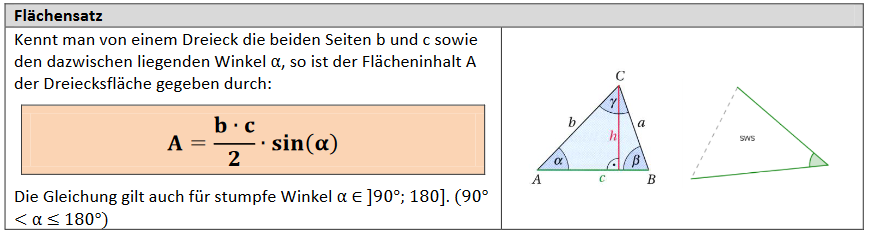
\includegraphics[scale=0.7]{flaechensatz.PNG}
\subsubsection{Berechnung am Kreissektor (auch Kreisausschnitt)}
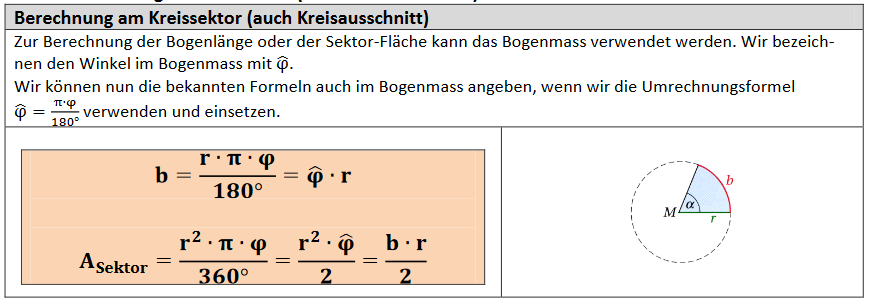
\includegraphics[scale=0.7]{kreissektor.PNG}
\subsubsection{Kreissegment (auch Kreisabschnitt)}
\includegraphics[scale=0.7]{kreissegment.PNG}



\subsection{Einheitskreis}
\subsubsection{Definition}
Der Einheitskreis ist ein Kreis um den Koordinatenursprung mit dem Radius r = 1 Laengeneinheit.
\subsubsection{Sinus- und Kosinusfunktion}
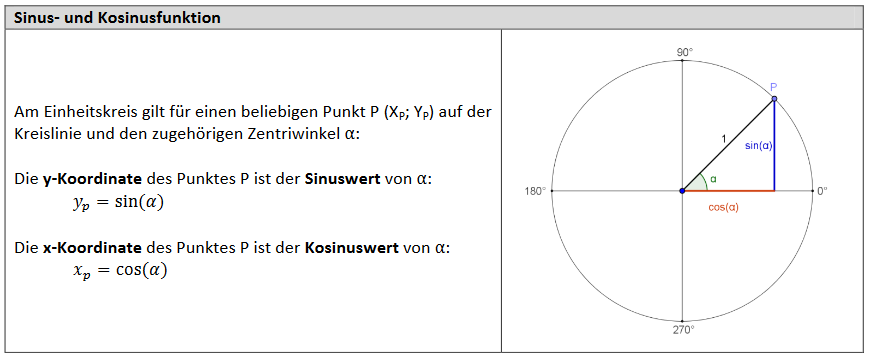
\includegraphics[scale=0.7]{einheitskreis1.PNG}
\subsubsection{Tangentsfunktion}
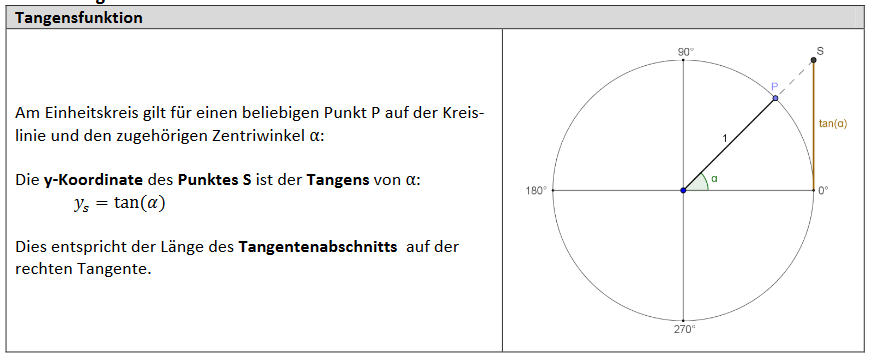
\includegraphics[scale=0.7]{einheitskreis2.PNG}
\subsubsection{Beziehungen zwischen den Winkelfunktionen (Phytagoras am Einheitskreis)}
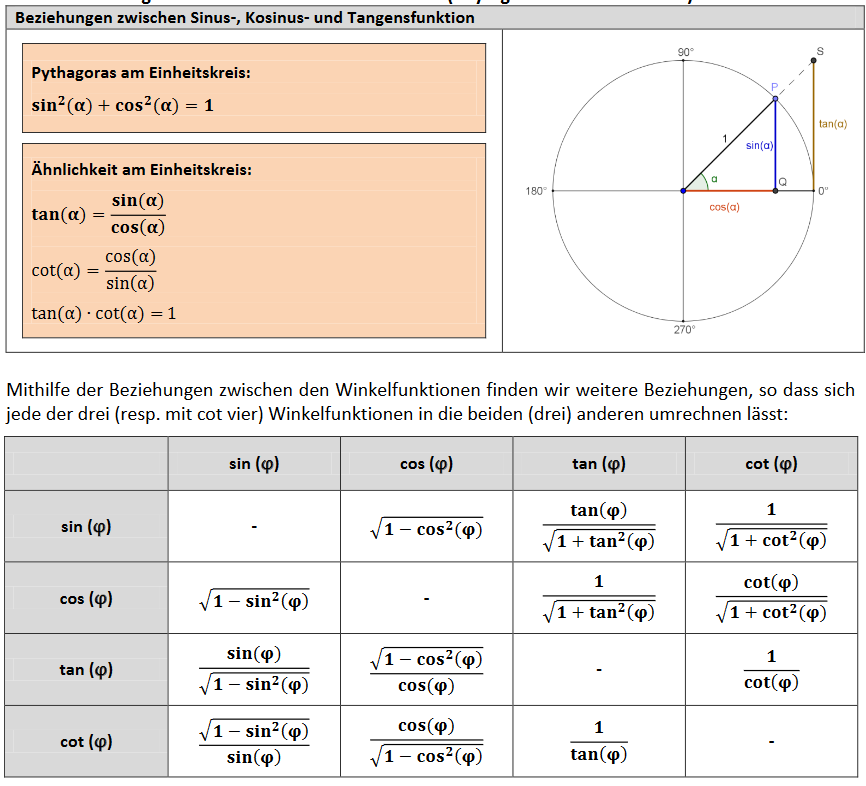
\includegraphics[scale=0.7]{einheitskreis3.PNG}
\subsubsection{Vorzeichen der Trigonometrischen Funktionen}
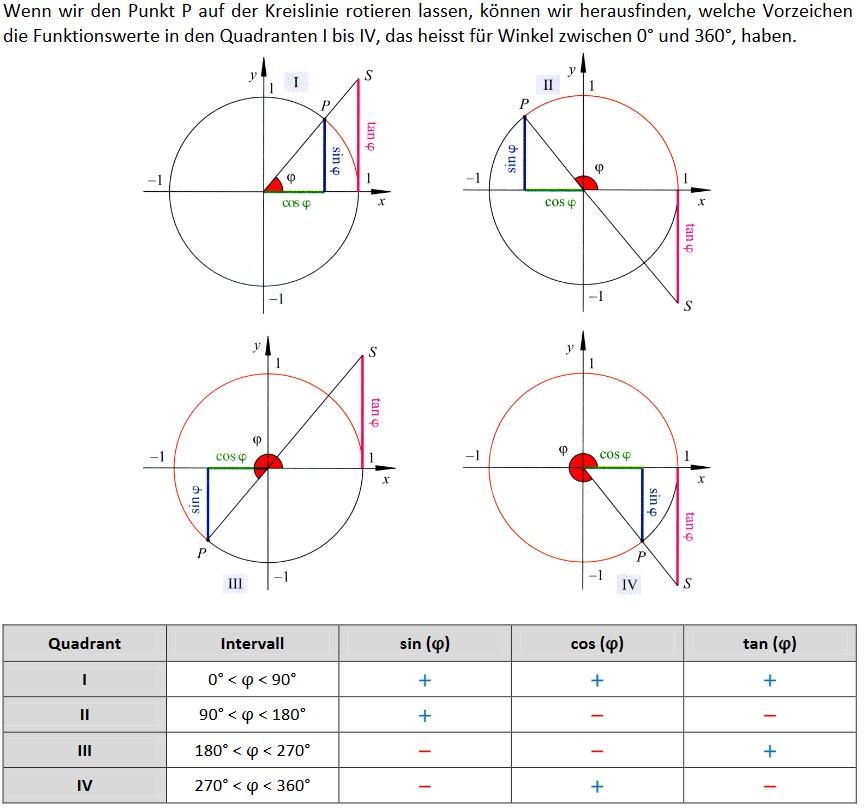
\includegraphics[scale=0.7]{einheitskreis4.PNG}

\subsection{Eigenschaften der Funktionen}
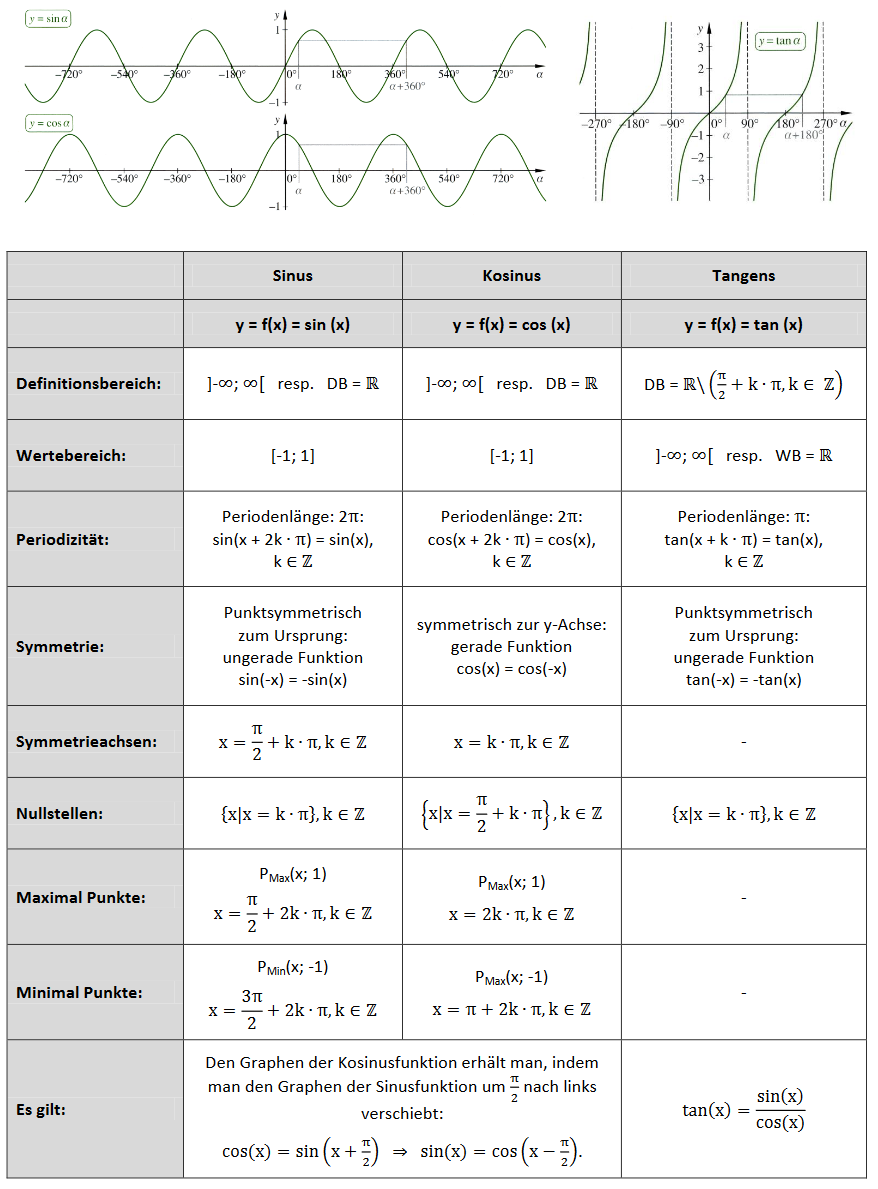
\includegraphics[scale=0.7]{trigfunktionen.PNG}

\subsection{Transformation der Sinusfunktion}
\subsubsection{Parameter a: Strecken. Stauchen auf der y-Achse (Amplitude)}
$y = a \cdot \sin(x)$ wobei $a \in \mathbb{R}\setminus0$ \\

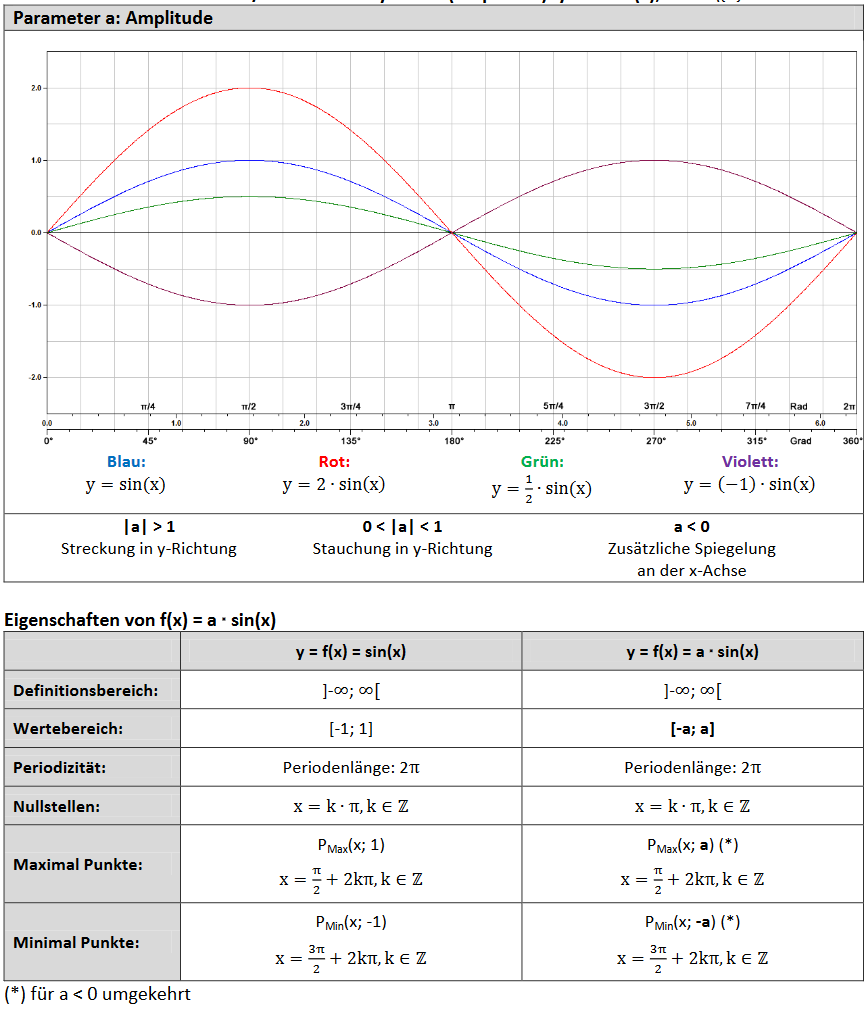
\includegraphics[scale=0.8]{sinus1.PNG}
\subsubsection{Eigenschaften von f(x) = a * sin(b * (x + u)) + v}
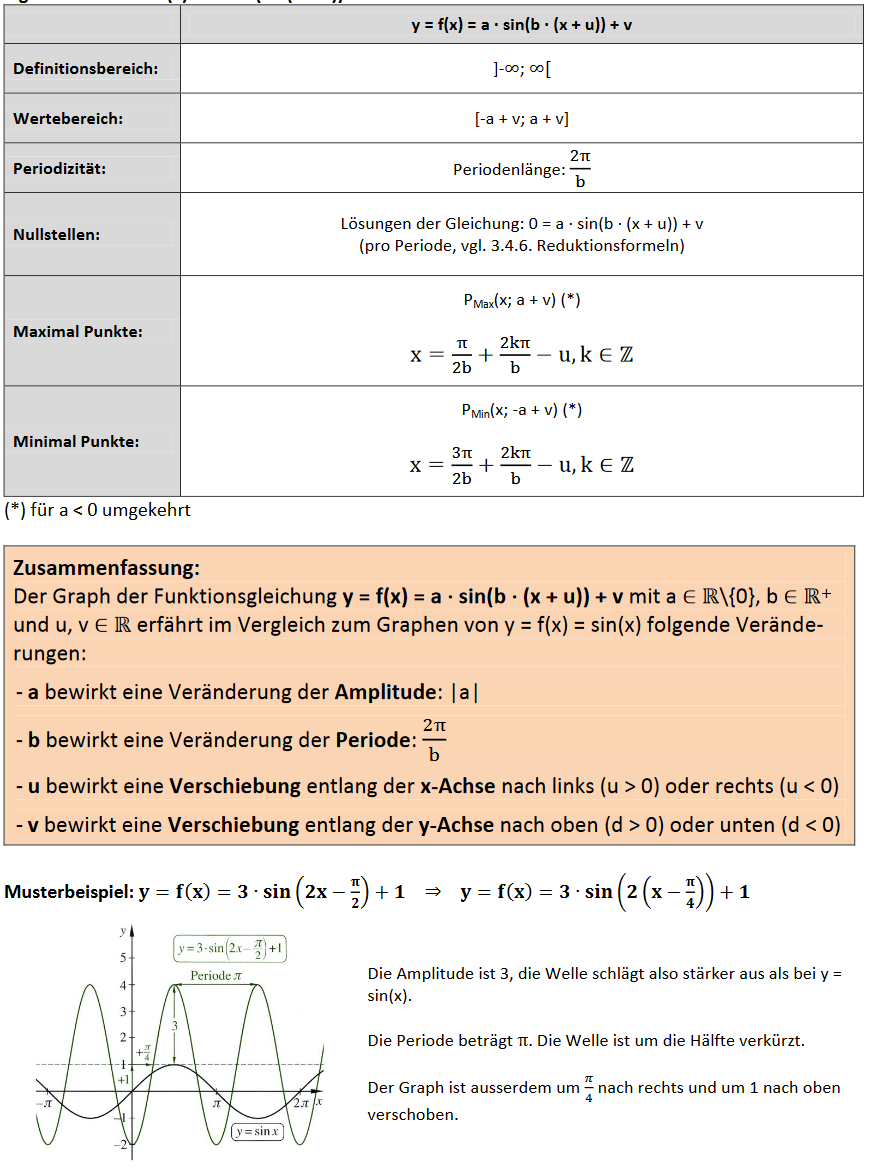
\includegraphics[scale=0.7 ]{sinmax.PNG}

\newpage{}
\section{Goniometrie}
\subsection{Grundlagen}
\subsubsection{Beziehungen}
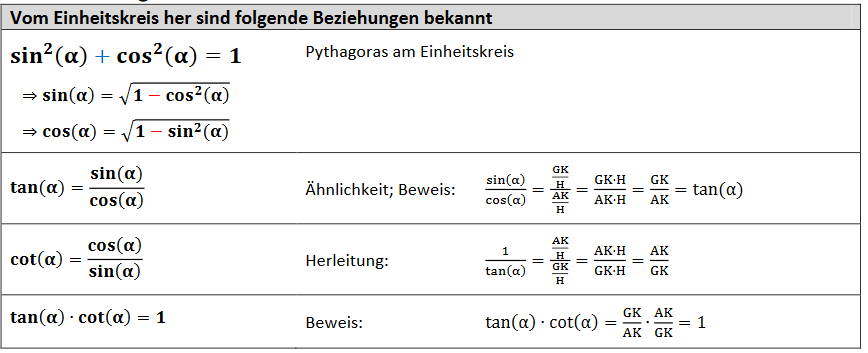
\includegraphics[scale=0.7]{gon1.PNG}

\subsubsection{Additionstheoreme}
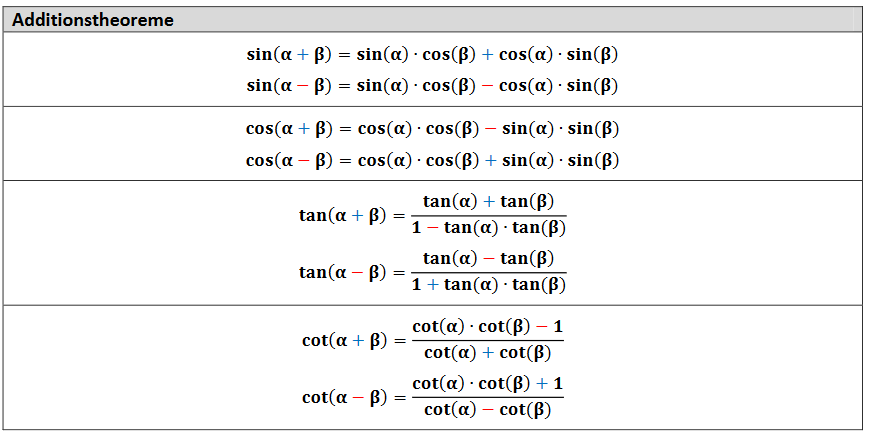
\includegraphics[scale=0.7]{gon2.PNG}

\subsubsection{Winkelfunktionen des doppelten Winkels}
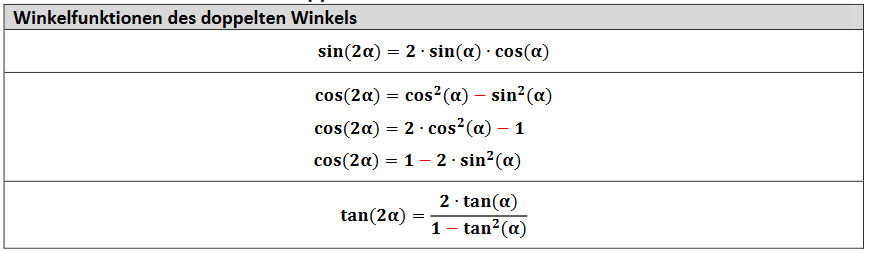
\includegraphics[scale=0.7]{gon3.PNG}

\subsubsection{Winkelfunktionen des dreifachen Winkels}
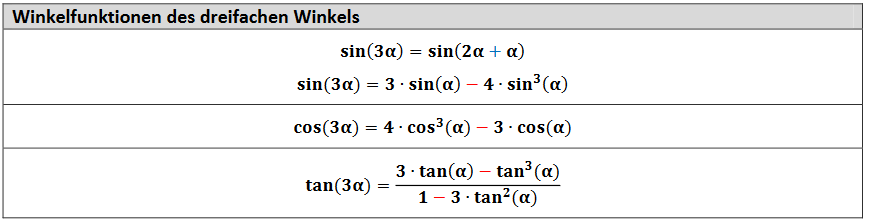
\includegraphics[scale=0.7]{gon4.PNG}

\subsubsection{Winkelfunktionen des halben Winkels}
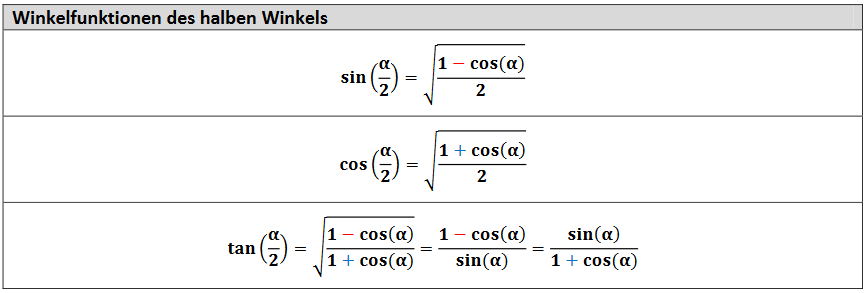
\includegraphics[scale=0.7]{gon5.PNG}

\section{Vektorgeometrie}
\textbf{Vektor:}

Ein Vektor ist festgelegt durch eine Laenge (Groesse) und eine Richtung.

\textbf{Freie Vektoren: }
Sie beschreiben Merkmale,
bei denen es nur auf Groesse und Richtung ankommt

\textbf{Ortsvektoren:}
Sie beschreiben Merkmale,
bei denen es auf Groesse, Richtung und Anfangspunkt ankommt

\subsection{Grunddefinitionen}
Unter einem Ortsvektor $\vec{v}$  versteht man eine Strecke, bei der der eine der beiden Begrenzungspunkte als Anfangspunkt P, der andere Endpunkt Q festgelegt ist. Man schreibt $\vec{v} = \vec{PQ}$

\subsection{Grundrechenarten}
\subsubsection{Addition von Vektoren}
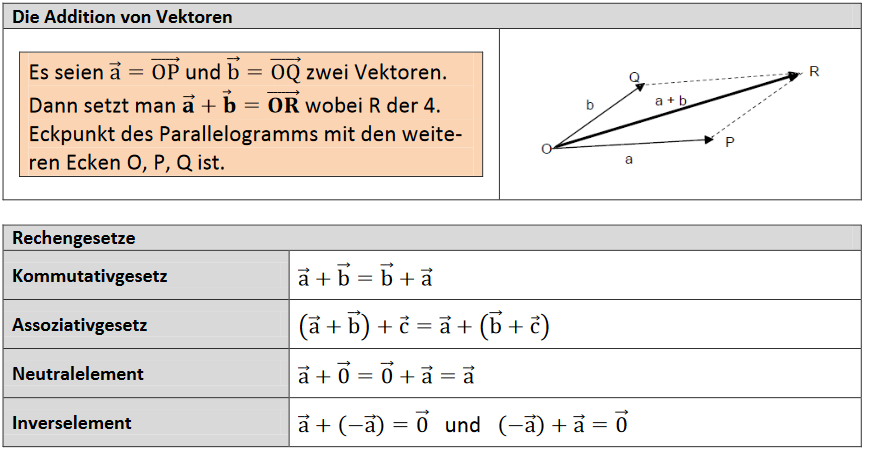
\includegraphics[scale=0.7]{vec1.PNG}
\subsubsection{Subtraktion von Vektoren}
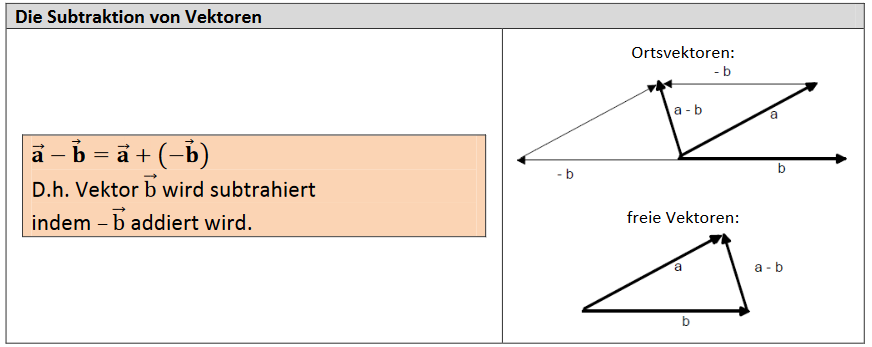
\includegraphics[scale=0.7]{vec2.PNG}
\subsubsection{Multiplikation mit einer Zahl}
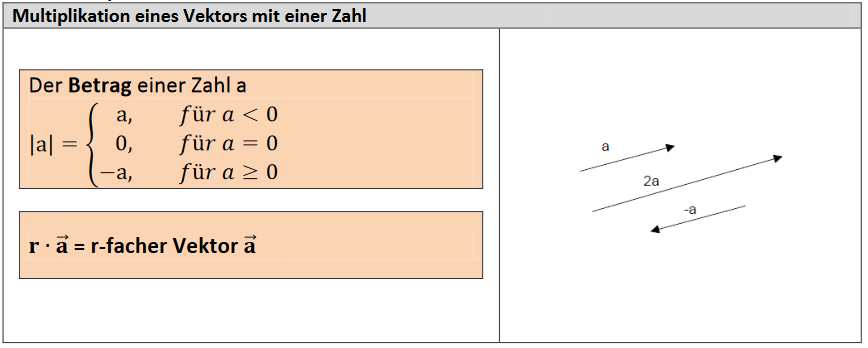
\includegraphics[scale=0.7]{vec3.PNG}

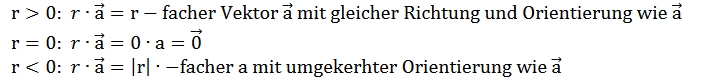
\includegraphics[scale=0.7]{vec3-1.PNG}

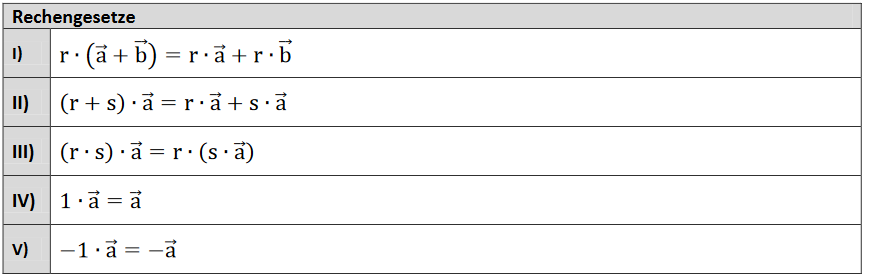
\includegraphics[scale=0.7]{vec3-2.PNG}

\subsubsection{Skalarprodukt}
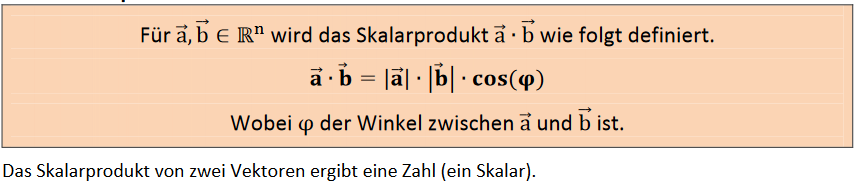
\includegraphics[scale=0.7]{vec4.PNG}

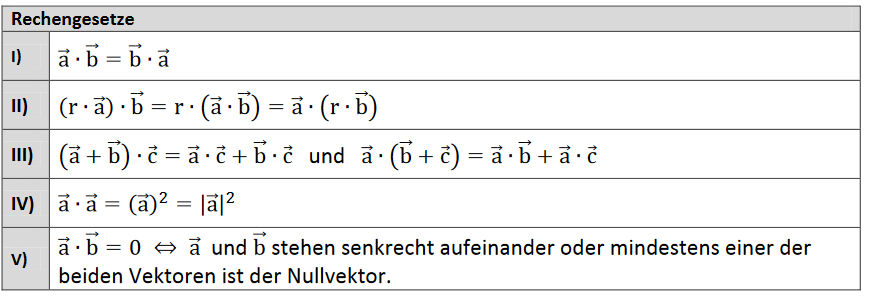
\includegraphics[scale=0.7]{vec4-1.PNG}

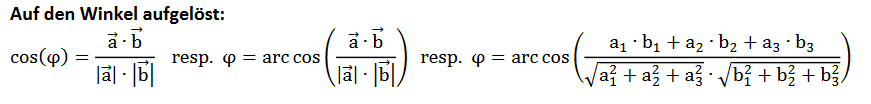
\includegraphics[scale=0.7]{vec4-2.PNG}

\subsubsection{Vektorprodukt}
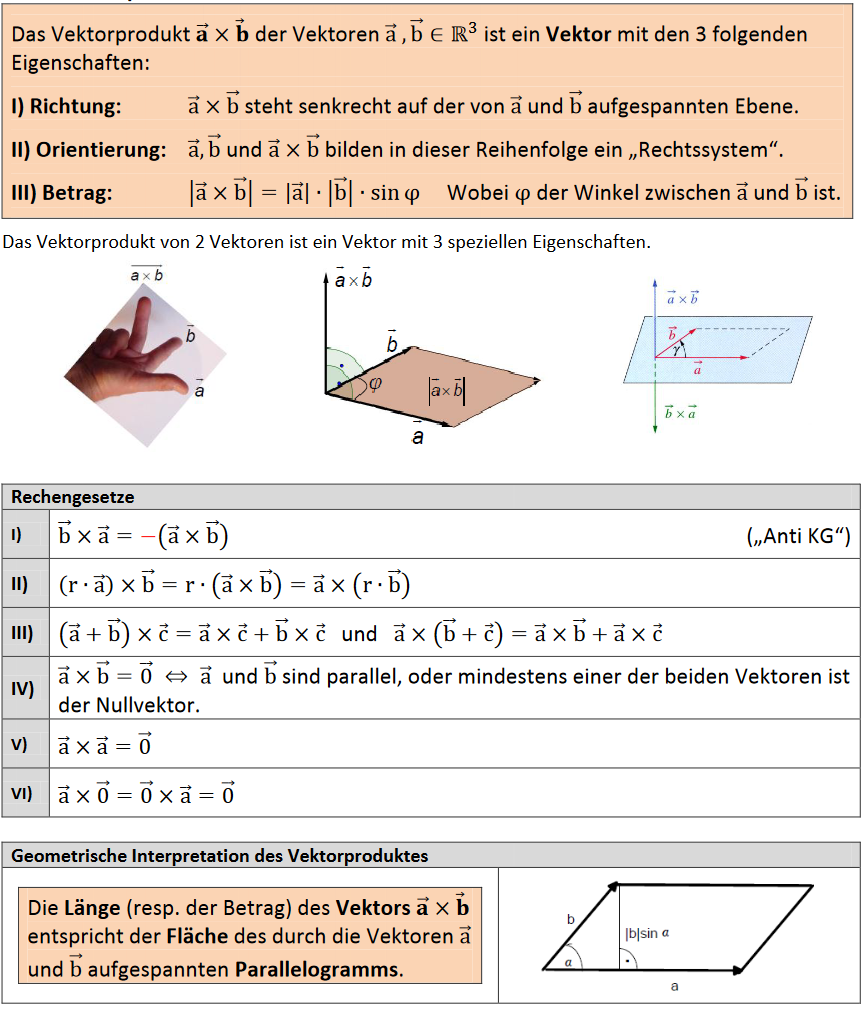
\includegraphics[scale=0.7]{vec5.PNG}
\newpage{}
\begin{multicols*}{2}
    \subsubsection{Betrag eines Vektors}
    Die Laenge eines Vektors heisst Betrag des Vektors.
    \[\vec{v}= \begin{pmatrix} x \\ y \end{pmatrix} \Longrightarrow \left|\vec{v}\right| = \sqrt{x^2 + y^2}\]
    \subsubsection{Einheitsvektor}
    Ein Vektor der Laenge heisst Einheitsvektor. \\
    Die Formel für die Berechnung des Einheitsvektors $\vec{a}^0$ lautet:
    \[\vec{a}^0 = \frac{1}{|a|} \vec{a}\]

    \subsection{Normalform}
    \subsubsection{Normalform einer Gerade}
    Eine Gerade laesst sich lediglich im $\mathbb{R}^2$ in Normalenform darstellen, weil es im $\mathbb{R}^3$ keinen eindeutigen Normalenvektor gibt.
    \[g\colon\; \vec{n} \circ [\vec{x} - \vec{a}] = 0\]

    \begin{itemize}
        \item  $\vec{g}$: Bezeichnung der Gerade
        \item  $\vec{n}$: Normalenvektor (Vektor, der senkrecht auf der Gerade steht)
        \item  $\vec{a}$: Aufpunkt (oder: Stuetzvektor)
    \end{itemize}
    \subsubsection{Normalform einer Ebene}
    \[E\colon\; \vec{n} \circ [\vec{x} - \vec{a}] = 0\]

    \begin{itemize}
        \item  $\vec{E}$: Bezeichnung der Ebene
        \item  $\vec{n}$: Normalenvektor (Vektor, der senkrecht auf der Gerade steht)
        \item  $\vec{a}$: Aufpunkt (oder: Stuetzvektor)
    \end{itemize}
    \subsubsection{Hessesche Normalform einer Gerade}
    \[g\colon\; \vec{n}_0 \circ [\vec{x} - \vec{a}] = 0\]
    \begin{itemize}
        \item  $\vec{n}$: Normalenvektor (Vektor, der auf einer Gerade senkrecht steht)
        \item  $\vec{n}_0$: Normierter Normalenvektor (Normalenvektor der Länge 1) $\vec{n}_0 = \frac{\vec{n}}{|\vec{n}|}$
        \item  $|\vec{n}|$: Laenge des Normalenvektors
        \item  $\vec{a}$: Aufpunkt (oder: Stuetzvektor)
    \end{itemize}

    Gegeben sei die Gerade g in Normalenform mit

    \[g\colon\; \vec{n} \circ \left[\vec{x} - \vec{a}\right] = \begin{pmatrix} 4 \\ 3 \end{pmatrix} \circ \left[\begin{pmatrix} x_1 \\ x_2 \end{pmatrix} - \begin{pmatrix} 2 \\ 1 \end{pmatrix}\right] = 0\]
    Länge des Normalenvektors berechnen:
    \[ |\vec{n}| = \sqrt{4^2 + 3^2} = \sqrt{25} = 5\]
    Gerade in Hessescher Normalform aufstellen
    \[g\colon\; \frac{\vec{n}}{|\vec{n}|} \circ \left[\vec{x} - \vec{a}\right] = \frac{1}{5} \cdot \begin{pmatrix} 4 \\ 3 \end{pmatrix} \circ \left[\begin{pmatrix} x_1 \\ x_2 \end{pmatrix} - \begin{pmatrix} 2 \\ 1 \end{pmatrix}\right] = 0\]

    Oder Gegeben sei die Gerade n in Koordinatenform mit:
    \[g\colon\; 4x_1 - 3x_2 - 5 = 0\]
    Normalenvektor aus Koordinatenform herauslesen

    Die Koordinaten des Normalenvektors entsprechen den Koeffizienten von $x_1$ und $x_2$ in der Koordinatenform.
    \[\vec{n} = \begin{pmatrix} 4 \\ -3 \end{pmatrix}\]
    Laenge des Normalenvektors berechnen
    \[|\vec{n}| = \sqrt{4^2 + (-3)^2} = \sqrt{25} = 5\]
    Gerade in Hessescher Normalform aufstellen
    \[g\colon\; \frac{1}{5} \cdot [4x_1 - 3x_2 - 5] = 0\]

    \subsubsection{Hessesche Normalform einer Ebene}
    \[E\colon\; \vec{n}_0 \circ [\vec{x} - \vec{a}] = 0\]
    \begin{itemize}
        \item  $\vec{n}$: Normalenvektor (Vektor, der auf einer Ebene senkrecht steht)
        \item  $\vec{n}_0$: Normierter Normalenvektor (Normalenvektor der Länge 1) $\vec{n}_0 = \frac{\vec{n}}{|\vec{n}|}$
        \item  $|\vec{n}|$: Laenge des Normalenvektors
        \item  $\vec{a}$: Aufpunkt (oder: Stuetzvektor)
    \end{itemize}
    Gegeben sei die Ebene E in Normalenform mit
    \[E\colon\; \vec{n} \circ \left[\vec{x} - \vec{a}\right] = \begin{pmatrix} 2 \\ 1 \\ -2 \end{pmatrix} \circ \left[\begin{pmatrix} x_1 \\ x_2 \\ x_3 \end{pmatrix} - \begin{pmatrix} 0 \\ 1 \\ 1 \end{pmatrix}\right] = 0\]
    Laenge des Normalenvektors berechnen
    \[|\vec{n}| = \sqrt{2^2 + 1^2 + (-2)^2} = \sqrt{9} = 3\]
    Ebene in Hessescher Normalform aufstellen
    \[E\colon\; \frac{\vec{n}}{|\vec{n}|} \circ \left[\vec{x} - \vec{a}\right] = \frac{1}{3} \cdot \begin{pmatrix} 2 \\ 1 \\ -2 \end{pmatrix} \circ \left[\begin{pmatrix} x_1 \\ x_2 \\ x_3 \end{pmatrix} - \begin{pmatrix} 0 \\ 1 \\ 1 \end{pmatrix}\right] = 0\]

\end{multicols*}

\newpage{}
